\begin{example}[Proposition 1 : $n = 6, \mathcal{PF'}_n \to \mathcal{D}_n$]
    ~\
    \begin{itemize}
        \item $f = (1, 1, 2, 4, 5, 5)$
            \subitem $l_1 = 2$
            \hspace{2cm} $l_2 = 1$
            \hspace{2cm} $l_3 = 0$
            \subitem $l_4 = 1$
            \hspace{2cm} $l_5 = 2$
            \hspace{2cm} $l_6 = 0$
        \item $w = (110100101100)$
    \end{itemize}
        \begin{center}
        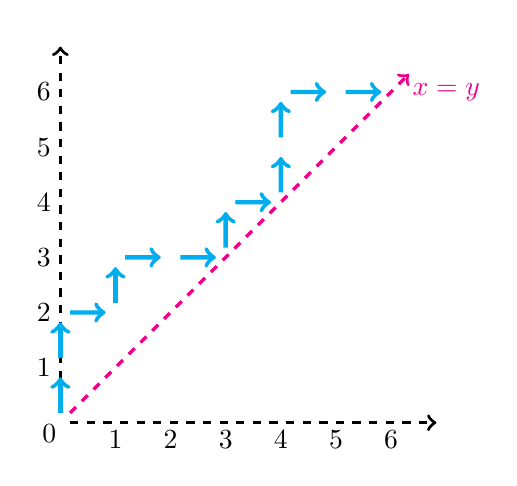
\begin{tikzpicture}[scale=0.7]
            \node (a) at (0, 0) {};
            \node (b) at (0, 7) {};
            \node (c) at (7, 0) {};
            \node (d) at (6.5, 6.5) {};
            \node (e) at (7, 6) [color = magenta]
                {$x = y$}; 
            \draw [dashed, very thick, ->] (a) to (b);
            \draw [dashed, very thick, ->] (a) to (c);
            \draw [dashed, very thick, ->]
                [color = magenta] (a) to (d);

            \node (1)  at (0,0)   {};
            \node (2)  at (0,1)   {};
            \node (3)  at (0,2)   {};
            \node (4)  at (1,2)   {};
            \node (5)  at (1,3)   {};
            \node (6)  at (2,3)   {};
            \node (7)  at (3,3)   {};
            \node (8)  at (3,4)   {};
            \node (9)  at (4,4)   {};
            \node (10) at (4,5)   {};
            \node (11) at (4,6)   {};
            \node (12) at (5,6)   {};
            \node (13) at (6,6)   {};
            \draw [->, ultra thick, color = cyan]
                (1)  to (2);
            \draw [->, ultra thick, color = cyan] 
                (2)  to (3);
            \draw [->, ultra thick, color = cyan]
                (3)  to (4);
            \draw [->, ultra thick, color = cyan]
                (4)  to (5);
            \draw [->, ultra thick, color = cyan]
                (5)  to (6);
            \draw [->, ultra thick, color = cyan]
                (6)  to (7);
            \draw [->, ultra thick, color = cyan]
                (7)  to (8);
            \draw [->, ultra thick, color = cyan]
                (8)  to (9);
            \draw [->, ultra thick, color = cyan]
                (9)  to (10);
            \draw [->, ultra thick, color = cyan]
                (10) to (11);
            \draw [->, ultra thick, color = cyan]
                (11) to (12);
            \draw [->, ultra thick, color = cyan]
                (12) to (13);

            \node at (-0.2, -0.2) {$0$};
            \node at (-0.3, 1)    {$1$};
            \node at (1, -0.3)    {$1$};
            \node at (-0.3, 2)    {$2$};
            \node at (2, -0.3)    {$2$};
            \node at (-0.3, 3)    {$3$};
            \node at (3, -0.3)    {$3$};
            \node at (-0.3, 4)    {$4$};
            \node at (4, -0.3)    {$4$};
            \node at (-0.3, 5)    {$5$};
            \node at (5, -0.3)    {$5$};
            \node at (-0.3, 6)    {$6$};
            \node at (6, -0.3)    {$6$};

        \end{tikzpicture}
    \end{center}
\end{example}

\begin{example}[Proposition 1 : $n = 6, \mathcal{D}_n \to \mathcal{PF'}_n$]
    ~\
    \begin{itemize}
        \item $w = 101011010010$
    \end{itemize}
    
    \begin{center}
        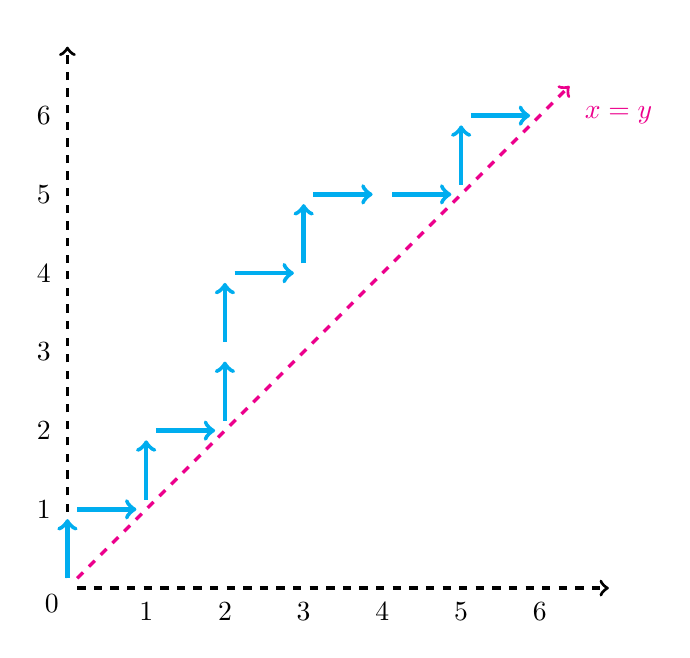
\begin{tikzpicture}[scale=1]
            \node (a) at (0, 0) {};
            \node (b) at (0, 7) {};
            \node (c) at (7, 0) {};
            \node (d) at (6.5, 6.5) {};
            \node (e) at (7, 6) [color = magenta]
                {$x = y$}; 
            \draw [dashed, very thick, ->] (a) to (b);
            \draw [dashed, very thick, ->] (a) to (c);
            \draw [dashed, very thick, ->]
                [color = magenta] (a) to (d);

            \node (1)  at (0,0)   {};
            \node (2)  at (0,1)   {};
            \node (3)  at (1,1)   {};
            \node (4)  at (1,2)   {};
            \node (5)  at (2,2)   {};
            \node (6)  at (2,3)   {};
            \node (7)  at (2,4)   {};
            \node (8)  at (3,4)   {};
            \node (9)  at (3,5)   {};
            \node (10) at (4,5)   {};
            \node (11) at (5,5)   {};
            \node (12) at (5,6)   {};
            \node (13) at (6,6)   {};
            \draw [->, ultra thick, color = cyan]
                (1)  to (2);
            \draw [->, ultra thick, color = cyan] 
                (2)  to (3);
            \draw [->, ultra thick, color = cyan]
                (3)  to (4);
            \draw [->, ultra thick, color = cyan]
                (4)  to (5);
            \draw [->, ultra thick, color = cyan]
                (5)  to (6);
            \draw [->, ultra thick, color = cyan]
                (6)  to (7);
            \draw [->, ultra thick, color = cyan]
                (7)  to (8);
            \draw [->, ultra thick, color = cyan]
                (8)  to (9);
            \draw [->, ultra thick, color = cyan]
                (9)  to (10);
            \draw [->, ultra thick, color = cyan]
                (10) to (11);
            \draw [->, ultra thick, color = cyan]
                (11) to (12);
            \draw [->, ultra thick, color = cyan]
                (12) to (13);

            \node at (-0.2, -0.2) {$0$};
            \node at (-0.3, 1)    {$1$};
            \node at (1, -0.3)    {$1$};
            \node at (-0.3, 2)    {$2$};
            \node at (2, -0.3)    {$2$};
            \node at (-0.3, 3)    {$3$};
            \node at (3, -0.3)    {$3$};
            \node at (-0.3, 4)    {$4$};
            \node at (4, -0.3)    {$4$};
            \node at (-0.3, 5)    {$5$};
            \node at (5, -0.3)    {$5$};
            \node at (-0.3, 6)    {$6$};
            \node at (6, -0.3)    {$6$};

        \end{tikzpicture}
    \end{center}
    \begin{itemize}
        \item Distances : 
            \subitem $s_1 = 0$
                \hspace{2cm} $a_1 = 1$
            \subitem $s_2 = 1$
                \hspace{2cm} $a_2 = 2$
            \subitem $s_3 = 2$
                \hspace{2cm} $a_3 = 3$
            \subitem $s_4 = 2$
                \hspace{2cm} $a_4 = 3$
            \subitem $s_5 = 3$
                \hspace{2cm} $a_5 = 4$
            \subitem $s_6 = 5$
                \hspace{2cm} $a_6 = 6$
        \item $f = (1, 2, 3, 3, 4, 6)$
    \end{itemize}
    
\end{example}

\begin{example}[Définition 5 : $n = 7$]
    $10110011001100 \gtrdot_d 10110101001100$
    \begin{itemize}
        \item $w_1 = 10110$
        \item $w_2 = 1001100$
    \end{itemize}
    \begin{center}
    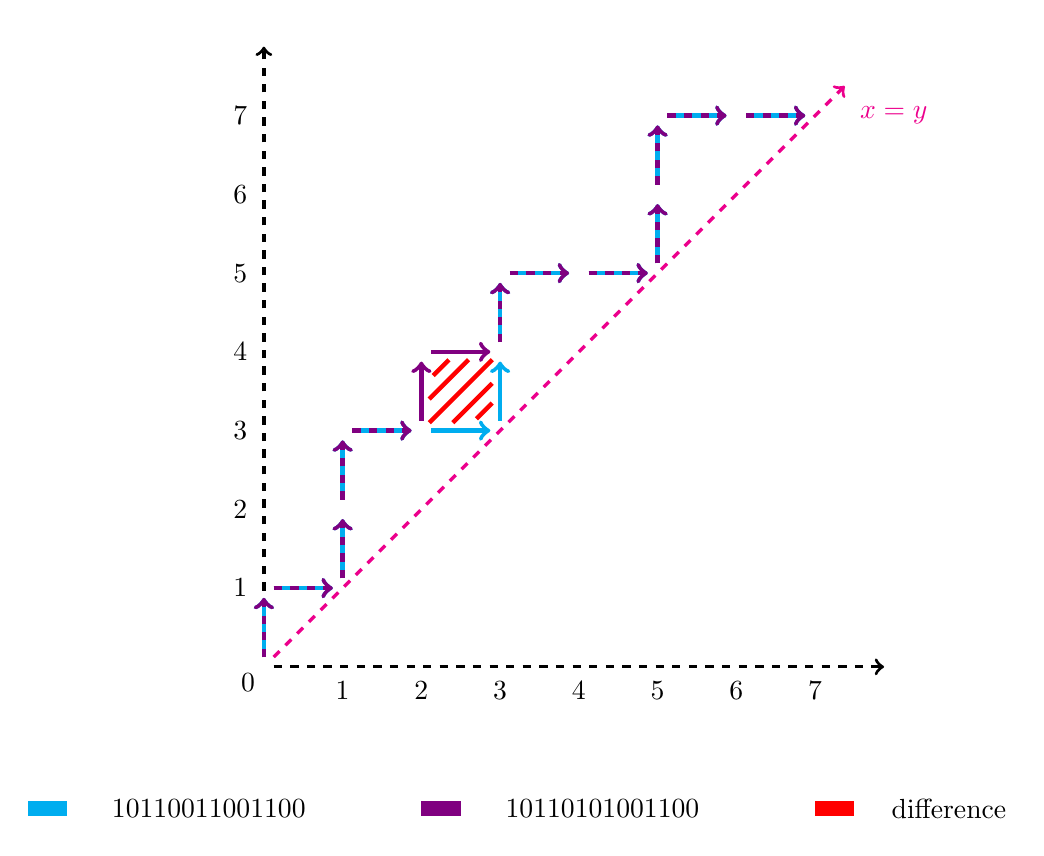
\begin{tikzpicture}[scale=1]
        \node (a) at (0, 0) {};
        \node (b) at (0, 8) {};
        \node (c) at (8, 0) {};
        \node (d) at (7.5, 7.5) {};
        \node (e) at (8, 7) [color = magenta]
            {$x = y$}; 
        \draw [dashed, very thick, ->] (a) to (b);
        \draw [dashed, very thick, ->] (a) to (c);
        \draw [dashed, very thick, ->]
            [color = magenta] (a) to (d);

        \node (1)  at (0,0)   {};
        \node (2)  at (0,1)   {};
        \node (3)  at (1,1)   {};
        \node (4)  at (1,2)   {};
        \node (5)  at (1,3)   {};
        \node (6)  at (2,3)   {};
        \node (7)  at (3,3)   {};
        \node (7b) at (2,4)   {};
        \node (8)  at (3,4)   {};
        \node (9)  at (3,5)   {};
        \node (10) at (4,5)   {};
        \node (11) at (5,5)   {};
        \node (12) at (5,6)   {};
        \node (13) at (5,7)   {};
        \node (14) at (6,7)   {};
        \node (15) at (7,7)   {};

        \draw [->, ultra thick, color = cyan]
            (1)  to (2);
        \draw [->, ultra thick, color = cyan] 
            (2)  to (3);
        \draw [->, ultra thick, color = cyan]
            (3)  to (4);
        \draw [->, ultra thick, color = cyan]
            (4)  to (5);
        \draw [->, ultra thick, color = cyan]
            (5)  to (6);
        \draw [->, ultra thick, color = cyan]
            (6)  to (7);
        \draw [->, ultra thick, color = cyan]
            (7)  to (8);
        \draw [->, ultra thick, color = cyan]
            (8)  to (9);
        \draw [->, ultra thick, color = cyan]
            (9)  to (10);
        \draw [->, ultra thick, color = cyan]
            (10) to (11);
        \draw [->, ultra thick, color = cyan]
            (11) to (12);
        \draw [->, ultra thick, color = cyan]
            (12) to (13);
        \draw [->, ultra thick, color = cyan]
            (13) to (14);
        \draw [->, ultra thick, color = cyan]
            (14) to (15);

        \draw [->, dashed, ultra thick, color = violet]
            (1)  to (2);
        \draw [->, dashed, ultra thick, color = violet] 
            (2)  to (3);
        \draw [->, dashed, ultra thick, color = violet]
            (3)  to (4);
        \draw [->, dashed, ultra thick, color = violet]
            (4)  to (5);
        \draw [->, dashed, ultra thick, color = violet]
            (5)  to (6);
        \draw [->, ultra thick, color = violet]
            (6)  to (7b);
        \draw [->, ultra thick, color = violet]
            (7b)  to (8);
        \draw [->, dashed, ultra thick, color = violet]
            (8)  to (9);
        \draw [->, dashed, ultra thick, color = violet]
            (9)  to (10);
        \draw [->, dashed, ultra thick, color = violet]
            (10) to (11);
        \draw [->, dashed, ultra thick, color = violet]
            (11) to (12);
        \draw [->, dashed, ultra thick, color = violet]
            (12) to (13);
        \draw [->, dashed, ultra thick, color = violet]
            (13) to (14);
        \draw [->, dashed, ultra thick, color = violet]
            (14) to (15);

        \node at (-0.2, -0.2) {$0$};
        \node at (-0.3, 1)    {$1$};
        \node at (1, -0.3)    {$1$};
        \node at (-0.3, 2)    {$2$};
        \node at (2, -0.3)    {$2$};
        \node at (-0.3, 3)    {$3$};
        \node at (3, -0.3)    {$3$};
        \node at (-0.3, 4)    {$4$};
        \node at (4, -0.3)    {$4$};
        \node at (-0.3, 5)    {$5$};
        \node at (5, -0.3)    {$5$};
        \node at (-0.3, 6)    {$6$};
        \node at (6, -0.3)    {$6$};
        \node at (-0.3, 7)    {$7$};
        \node at (7, -0.3)    {$7$};

        \draw[color = red, ultra thick]
            (2.1,3.1) -- (2.9,3.9);
        \draw[color = red, ultra thick]
            (2.1,3.4) -- (2.6,3.9);
        \draw[color = red, ultra thick]
            (2.15,3.7) -- (2.35,3.9);
        \draw[color = red, ultra thick]
            (2.4,3.1) -- (2.9,3.6);
        \draw[color = red, ultra thick]
            (2.7,3.15) -- (2.9,3.35);

        \fill[color = cyan] (-3,-1.9) rectangle
            (-2.5,-1.7);
        \node at (-0.7,-1.8) {$10110011001100$};
        \fill[color = violet] (2,-1.9) rectangle
        (2.5,-1.7);
        \node at (4.3,-1.8) {$10110101001100$};
        \fill[color = red] (7,-1.9) rectangle
        (7.5,-1.7);
        \node at (8.7,-1.8) {difference};
    \end{tikzpicture}
\end{center}
\end{example}

\begin{example}[Définition 7 : $n = 6$]
    $(1, 1, 2, 3, 4, 5) \gtrdot (1, 1, 2, 3, 3, 5)$    
\end{example}

\begin{example}[Les posets de $\mathcal{D}_4$ et $\mathcal{PF'}_4$]
    ~\\
    \begin{center}
        \begin{center}
    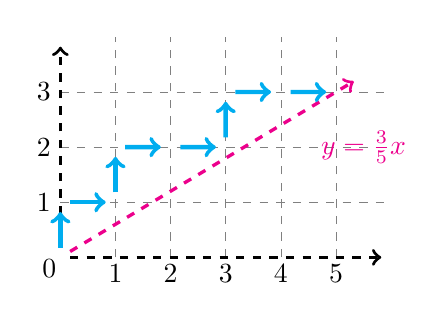
\begin{tikzpicture}[scale=0.7]
        \node (a) at (0, 0) {};
        \node (b) at (0, 4) {};
        \node (c) at (6, 0) {};
        \node (d) at (5.5, 3.3) {};

        \draw [dashed, very thin, color=gray] (1,0) to (1,4);
        \draw [dashed, very thin, color=gray] (2,0) to (2,4);
        \draw [dashed, very thin, color=gray] (3,0) to (3,4);
        \draw [dashed, very thin, color=gray] (4,0) to (4,4);
        \draw [dashed, very thin, color=gray] (5,0) to (5,4);
        \draw [dashed, very thin, color=gray] (0,1) to (6,1);
        \draw [dashed, very thin, color=gray] (0,2) to (6,2);
        \draw [dashed, very thin, color=gray] (0,3) to (6,3);
        
        \node (e) at (5.5, 2) [color = magenta] {$y = \frac{3}{5}x$}; 
        \draw [dashed, very thick, ->] (a) to (b);
        \draw [dashed, very thick, ->] (a) to (c);
        \draw [dashed, very thick, ->]
            [color = magenta] (a) to (d);

        \node (1)  at (0,0)   {};
        \node (2)  at (0,1)   {};
        \node (3)  at (1,1)   {};
        \node (4)  at (1,2)   {};
        \node (5)  at (2,2)   {};
        \node (6)  at (3,2)   {};
        \node (7)  at (3,3)   {};
        \node (8)  at (4,3)   {};
        \node (9)  at (5,3)   {};
        \draw [->, ultra thick, color = cyan]
            (1)  to (2);
        \draw [->, ultra thick, color = cyan] 
            (2)  to (3);
        \draw [->, ultra thick, color = cyan]
            (3)  to (4);
        \draw [->, ultra thick, color = cyan]
            (4)  to (5);
        \draw [->, ultra thick, color = cyan]
            (5)  to (6);
        \draw [->, ultra thick, color = cyan]
            (6)  to (7);
        \draw [->, ultra thick, color = cyan]
            (7)  to (8);
        \draw [->, ultra thick, color = cyan]
            (8)  to (9);

        \node at (-0.2, -0.2) {$0$};
        \node at (-0.3, 1)    {$1$};
        \node at (1, -0.3)    {$1$};
        \node at (-0.3, 2)    {$2$};
        \node at (2, -0.3)    {$2$};
        \node at (-0.3, 3)    {$3$};
        \node at (3, -0.3)    {$3$};
        \node at (4, -0.3)    {$4$};
        \node at (5, -0.3)    {$5$};

    \end{tikzpicture}
\end{center}
        Ces posets contiennent chacun $\frac {1}{5} \binom{8}{4} =
        14$ éléments.
    \end{center}
\end{example}


\begin{example}[Proposition 3 : $n = 6, \mathcal{PF}_n \to \mathcal{LD}_n$]
    ~\
    \begin{itemize}
        \item $f = (5, 2, 1, 4, 5, 1)$
            \subitem $im_1 = \{3, 6\}$
            \hspace{16mm} $im_2 = \{2\}$
            \hspace{24mm} $im_3 = \emptyset$
            \subitem $im_4 = \{4\}$
            \hspace{2cm} $im_5 = \{1, 5\}$
            \hspace{2cm} $im_6 = \emptyset$
        \item $w = 360200401500$
    \end{itemize}
    \begin{center}
    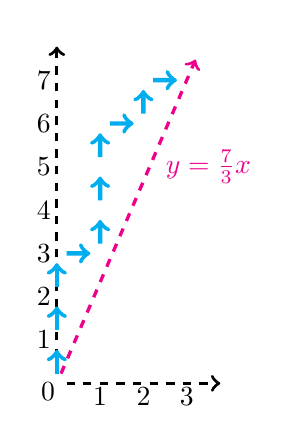
\begin{tikzpicture}[scale=0.55]
        \node (a) at (0, 0) {};
        \node (b) at (0, 8) {};
        \node (c) at (4, 0) {};
        \node (d) at (3.3, 7.7) {};
        \node (e) at (3.5, 5) [color = magenta]
            {$y = \frac{7}{3}x$}; 
        \draw [dashed, very thick, ->] (a) to (b);
        \draw [dashed, very thick, ->] (a) to (c);
        \draw [dashed, very thick, ->]
            [color = magenta] (a) to (d);

        \node (1)  at (0,0)   {};
        \node (2)  at (0,1)   {};
        \node (3)  at (0,2)   {};
        \node (4)  at (0,3)   {};
        \node (5)  at (1,3)   {};
        \node (6)  at (1,4)   {};
        \node (7)  at (1,5)   {};
        \node (8)  at (1,6)   {};
        \node (9)  at (2,6)   {};
        \node (10) at (2,7)   {};
        \node (11) at (3,7)   {};
        \draw [->, ultra thick, color = cyan]
            (1)  to (2);
        \draw [->, ultra thick, color = cyan] 
            (2)  to (3);
        \draw [->, ultra thick, color = cyan]
            (3)  to (4);
        \draw [->, ultra thick, color = cyan]
            (4)  to (5);
        \draw [->, ultra thick, color = cyan]
            (5)  to (6);
        \draw [->, ultra thick, color = cyan]
            (6)  to (7);
        \draw [->, ultra thick, color = cyan]
            (7)  to (8);
        \draw [->, ultra thick, color = cyan]
            (8)  to (9);
        \draw [->, ultra thick, color = cyan]
            (9)  to (10);
        \draw [->, ultra thick, color = cyan]
            (10) to (11);

        \node at (-0.2, -0.2) {$0$};
        \node at (-0.3, 1)    {$1$};
        \node at (1, -0.3)    {$1$};
        \node at (-0.3, 2)    {$2$};
        \node at (2, -0.3)    {$2$};
        \node at (-0.3, 3)    {$3$};
        \node at (3, -0.3)    {$3$};
        \node at (-0.3, 4)    {$4$};
        \node at (-0.3, 5)    {$5$};
        \node at (-0.3, 6)    {$6$};
        \node at (-0.3, 7)    {$7$};

    \end{tikzpicture}
\end{center}
\end{example}

\begin{example}[Proposition 3 : $n = 6, \mathcal{LD}_n \to \mathcal{PF}_n$]
    ~\
    \begin{itemize}
        \item $w = 402560010030$
    \end{itemize}
    \begin{center}
    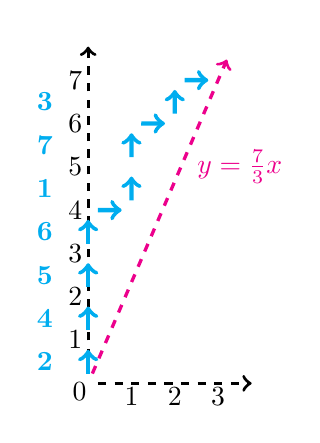
\begin{tikzpicture}[scale=0.55]
        \node (a) at (0, 0) {};
        \node (b) at (0, 8) {};
        \node (c) at (4, 0) {};
        \node (d) at (3.3, 7.7) {};
        \node (e) at (3.5, 5) [color = magenta]
            {$y = \frac{7}{3}x$}; 
        \draw [dashed, very thick, ->] (a) to (b);
        \draw [dashed, very thick, ->] (a) to (c);
        \draw [dashed, very thick, ->]
            [color = magenta] (a) to (d);

        \node (1)  at (0,0)   {};
        \node (2)  at (0,1)   {};
        \node (3)  at (0,2)   {};
        \node (4)  at (0,3)   {};
        \node (5)  at (0,4)   {};
        \node (6)  at (1,4)   {};
        \node (7)  at (1,5)   {};
        \node (8)  at (1,6)   {};
        \node (9)  at (2,6)   {};
        \node (10) at (2,7)   {};
        \node (11) at (3,7)   {};
        \draw [->, ultra thick, color = cyan]
            (1)  to (2);
        \draw [->, ultra thick, color = cyan] 
            (2)  to (3);
        \draw [->, ultra thick, color = cyan]
            (3)  to (4);
        \draw [->, ultra thick, color = cyan]
            (4)  to (5);
        \draw [->, ultra thick, color = cyan]
            (5)  to (6);
        \draw [->, ultra thick, color = cyan]
            (6)  to (7);
        \draw [->, ultra thick, color = cyan]
            (7)  to (8);
        \draw [->, ultra thick, color = cyan]
            (8)  to (9);
        \draw [->, ultra thick, color = cyan]
            (9)  to (10);
        \draw [->, ultra thick, color = cyan]
            (10) to (11);

        \node at (-0.2, -0.2) {$0$};
        \node at (-0.3, 1)    {$1$};
        \node at (1, -0.3)    {$1$};
        \node at (-0.3, 2)    {$2$};
        \node at (2, -0.3)    {$2$};
        \node at (-0.3, 3)    {$3$};
        \node at (3, -0.3)    {$3$};
        \node at (-0.3, 4)    {$4$};
        \node at (-0.3, 5)    {$5$};
        \node at (-0.3, 6)    {$6$};
        \node at (-0.3, 7)    {$7$};

        \node [color = cyan] at (-1, 0.5) {\textbf{2}};
        \node [color = cyan] at (-1, 1.5) {\textbf{4}};
        \node [color = cyan] at (-1, 2.5) {\textbf{5}};
        \node [color = cyan] at (-1, 3.5) {\textbf{6}};
        \node [color = cyan] at (-1, 4.5) {\textbf{1}};
        \node [color = cyan] at (-1, 5.5) {\textbf{7}};
        \node [color = cyan] at (-1, 6.5) {\textbf{3}};
    \end{tikzpicture}
\end{center}
    \begin{itemize}
        \item Distances :
            \subitem $s_1 = 0$
            \hspace{2cm} $s_2 = 1$
            \hspace{2cm} $s_3 = 1$
            \subitem $s_4 = 1$
            \hspace{2cm} $s_5 = 3$
            \hspace{2cm} $s_6 = 5$
        \item Labels :
            \subitem $dist_0 = \{4\}$
            \hspace{2cm} $dist_1 = \{2, 5, 6\}$
            \hspace{2cm} $dist_2 = \emptyset$
            \subitem $dist_3 = \{1\}$
            \hspace{2cm} $dist_4 = \emptyset$
            \hspace{32mm} $dist_5 = \{3\}$
        \item $f = (4, 2, 6, 1, 2, 2)$
    \end{itemize}
\end{example}

\begin{example}[Définition 8 : $n = 5$]
    $104503600200 \gtrdot_{ld} 10345060200$
    \begin{itemize}
        \item $l = 10$
        \item $r = 0200$
        \item $x = 45$
        \item $x' = 345$
        \item $y = 3$
        \item $z = 36$
        \item $z' = 6$
    \end{itemize}
    \begin{center}
    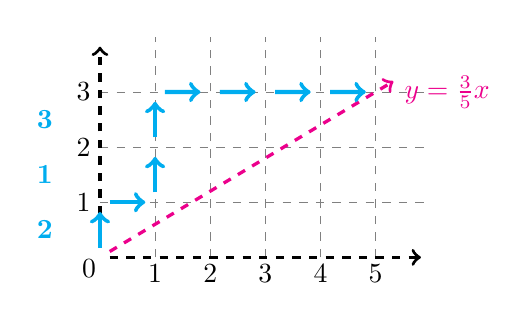
\begin{tikzpicture}[scale=0.7]
        \node (a) at (0, 0) {};
        \node (b) at (0, 4) {};
        \node (c) at (6, 0) {};
        \node (d) at (5.5, 3.3) {};

        \draw [dashed, very thin, color=gray] (1,0) to (1,4);
        \draw [dashed, very thin, color=gray] (2,0) to (2,4);
        \draw [dashed, very thin, color=gray] (3,0) to (3,4);
        \draw [dashed, very thin, color=gray] (4,0) to (4,4);
        \draw [dashed, very thin, color=gray] (5,0) to (5,4);
        \draw [dashed, very thin, color=gray] (0,1) to (6,1);
        \draw [dashed, very thin, color=gray] (0,2) to (6,2);
        \draw [dashed, very thin, color=gray] (0,3) to (6,3);

        \node (e) at (6.3, 3) [color = magenta] {$y = \frac{3}{5}x$}; 
        \draw [dashed, very thick, ->] (a) to (b);
        \draw [dashed, very thick, ->] (a) to (c);
        \draw [dashed, very thick, ->]
            [color = magenta] (a) to (d);

        \node (1)  at (0,0)   {};
        \node (2)  at (0,1)   {};
        \node (3)  at (1,1)   {};
        \node (4)  at (1,2)   {};
        \node (5)  at (1,3)   {};
        \node (6)  at (2,3)   {};
        \node (7)  at (3,3)   {};
        \node (8)  at (4,3)   {};
        \node (9)  at (5,3)   {};
        \draw [->, ultra thick, color = cyan]
            (1)  to (2);
        \draw [->, ultra thick, color = cyan] 
            (2)  to (3);
        \draw [->, ultra thick, color = cyan]
            (3)  to (4);
        \draw [->, ultra thick, color = cyan]
            (4)  to (5);
        \draw [->, ultra thick, color = cyan]
            (5)  to (6);
        \draw [->, ultra thick, color = cyan]
            (6)  to (7);
        \draw [->, ultra thick, color = cyan]
            (7)  to (8);
        \draw [->, ultra thick, color = cyan]
            (8)  to (9);

        \node at (-0.2, -0.2) {$0$};
        \node at (-0.3, 1)    {$1$};
        \node at (1, -0.3)    {$1$};
        \node at (-0.3, 2)    {$2$};
        \node at (2, -0.3)    {$2$};
        \node at (-0.3, 3)    {$3$};
        \node at (3, -0.3)    {$3$};
        \node at (4, -0.3)    {$4$};
        \node at (5, -0.3)    {$5$};

        \node [color = cyan] at (-1, 0.5) {\textbf{2}};
        \node [color = cyan] at (-1, 1.5) {\textbf{1}};
        \node [color = cyan] at (-1, 2.5) {\textbf{3}};
    \end{tikzpicture}
\end{center}
\end{example}